\documentclass{article}
\usepackage{graphicx}
\usepackage{enumitem}
\usepackage{algorithm}
\usepackage{algpseudocode}
\usepackage{caption}
\usepackage{amsthm}
\usepackage[margin=2cm]{geometry}

\pagestyle{empty}
\setlist{nosep}
\algnewcommand\algorithmicforeach{\textbf{for each}}
\algdef{S}[FOR]{ForEach}[1]{\algorithmicforeach\ #1\ \algorithmicdo}
\algnewcommand\algorithmicswitch{\textbf{switch}}
\algnewcommand\algorithmiccase{\textbf{case}}
\algdef{SE}[SWITCH]{Switch}{EndSwitch}[1]{\algorithmicswitch\ #1\ \algorithmicdo}{\algorithmicend\ \algorithmicswitch}%
\algdef{SE}[CASE]{Case}{EndCase}[1]{\algorithmiccase\ #1}{\algorithmicend\ \algorithmiccase}%
\algtext*{EndSwitch}%
\algtext*{EndCase}%
\newtheorem*{lemma}{Lemma}

\begin{document}
    \section*{Cell record}
    Cell:
    \begin{itemize}
        \item id: Int.  Unique cell identifier.
        \item lineage: String.  The branch of the cell in the quadtree.  It provides position and depth of the cell. 
        \item envelope: Polygon.  Geometric representation of the cell.
    \end{itemize}
    
    \section*{Lineage example}
    \begin{figure}[h!]\label{fig:lineage}
        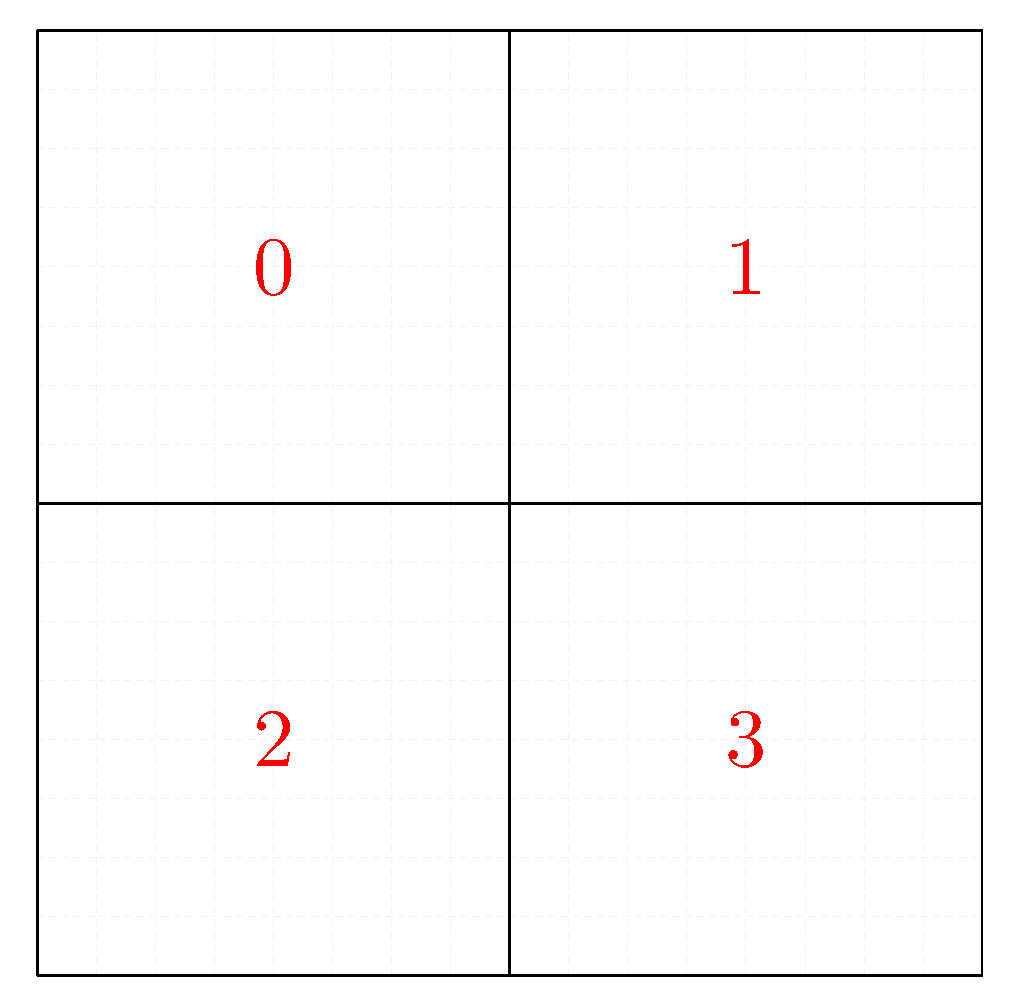
\includegraphics[page=1,width=0.32\linewidth]{Figures/Lineage}
        \includegraphics[page=2,width=0.32\linewidth]{Figures/Lineage}
        \includegraphics[page=3,width=0.32\linewidth]{Figures/Lineage}
        \caption{Lineage can provide the cell's position (string's last character) and its depth (string's length).}
    \end{figure}

    
    \section*{Algorithms}
    \begin{algorithm} \caption{\textsc{getNextCellWithEdges} algorithm}
        \textbf{Require:} a quadtree with cell envelopes $\mathcal Q$ and map of cells and their edge count $\mathcal M$.
        \begin{algorithmic}[1]
        \Function{ getNextCellWithEdges }{ $\mathcal Q$, $\mathcal M$ }
            \State $\mathcal C \gets $ list of empty cells in $\mathcal M$
            \ForEach{ $emptyCell$ in $\mathcal C $ }
                \State initialize $cellList$ with $emptyCell$ 
                \State $done \gets false$
                \Repeat
                    \State $c \gets $ last cell in $cellList$ 
                    \State $cells, corner \gets \textsc{getCellsInCorner}(\mathcal Q, c)$ \Comment{ return 3 cells and the reference corner }
                    \ForEach{$cell$ in $cells$}
                        \State check $cell$ in $\mathcal M$ \Comment{ using $cell.id$ }
                        \If{ $cell$ has edges }
                            \State \textbf{output} ($cellList$, $cell$, $corner$)
                            \State $done \gets true$
                        \EndIf
                    \EndFor
                    \If{ not $done$ }
                        \State $cells \gets$ sort $cells$ on basis of their depth \Comment{ using $cell.lineage$ }
                        \State add $cells$ to $cellList$
                    \EndIf
                \Until{ $done$ }
            \EndFor
        \EndFunction
        \end{algorithmic}
    \end{algorithm}
    
    \begin{algorithm} \caption{\textsc{getCellsInCorner} algorithm}
        \textbf{Require:} a quadtree with cell envelopes $\mathcal Q$ and a cell $c$.
        \begin{algorithmic}[1]
        \Function{ getCellsInCorner }{ $\mathcal Q$, $c$ }
            \State $region \gets $ last character in $c.lineage$
            \Switch{ $region$ }
                \Case{ `0' }
                    \State $corner \gets$ left bottom corner of $c.envelope$
                \EndCase
                \Case{ `1' }
                    \State $corner \gets$ right bottom corner of $c.envelope$
                \EndCase
                \Case{ `2' }
                    \State $corner \gets$ left upper corner of $c.envelope$
                \EndCase
                \Case{ `3' }
                    \State $corner \gets$ right upper corner of $c.envelope$
                \EndCase
            \EndSwitch
            \State $cells \gets$ cells which intersect $corner$ in $\mathcal Q$
            \State $cells \gets cells - c$ \Comment{ Remove the current cell from the intersected cells }
            \State \Return{ ($cells$, $corner$) }
        \EndFunction
        \end{algorithmic}
    \end{algorithm}
    
    \begin{lemma}
    Four cells at the same level can not be empty.  At least one of them must have edges in order to force the split.
    \end{lemma}
    
    \begin{proof}
    The $\textsc{getCellsInCorner}$ function will query the interior corner of a cell according to its position, that is the centroid of its cell parent.  The only cells which can intersect that point are cells at the same level of the current cell or their children.  If the 3 cells returned by $\textsc{getCellsInCorner}$ are empty, at least one of them must have a deeper level that the current cell.  Following that cell guarantees that the search space will be shrank at each iteration.  Eventually, the algorithm will reach the maximum level of the quadtree where all the involved cells will have the same level and, therefore, at least one of them must have edges.
    \end{proof}
    
    \section*{Algorithms example}
    \begin{figure}[!ht]
        \centering
        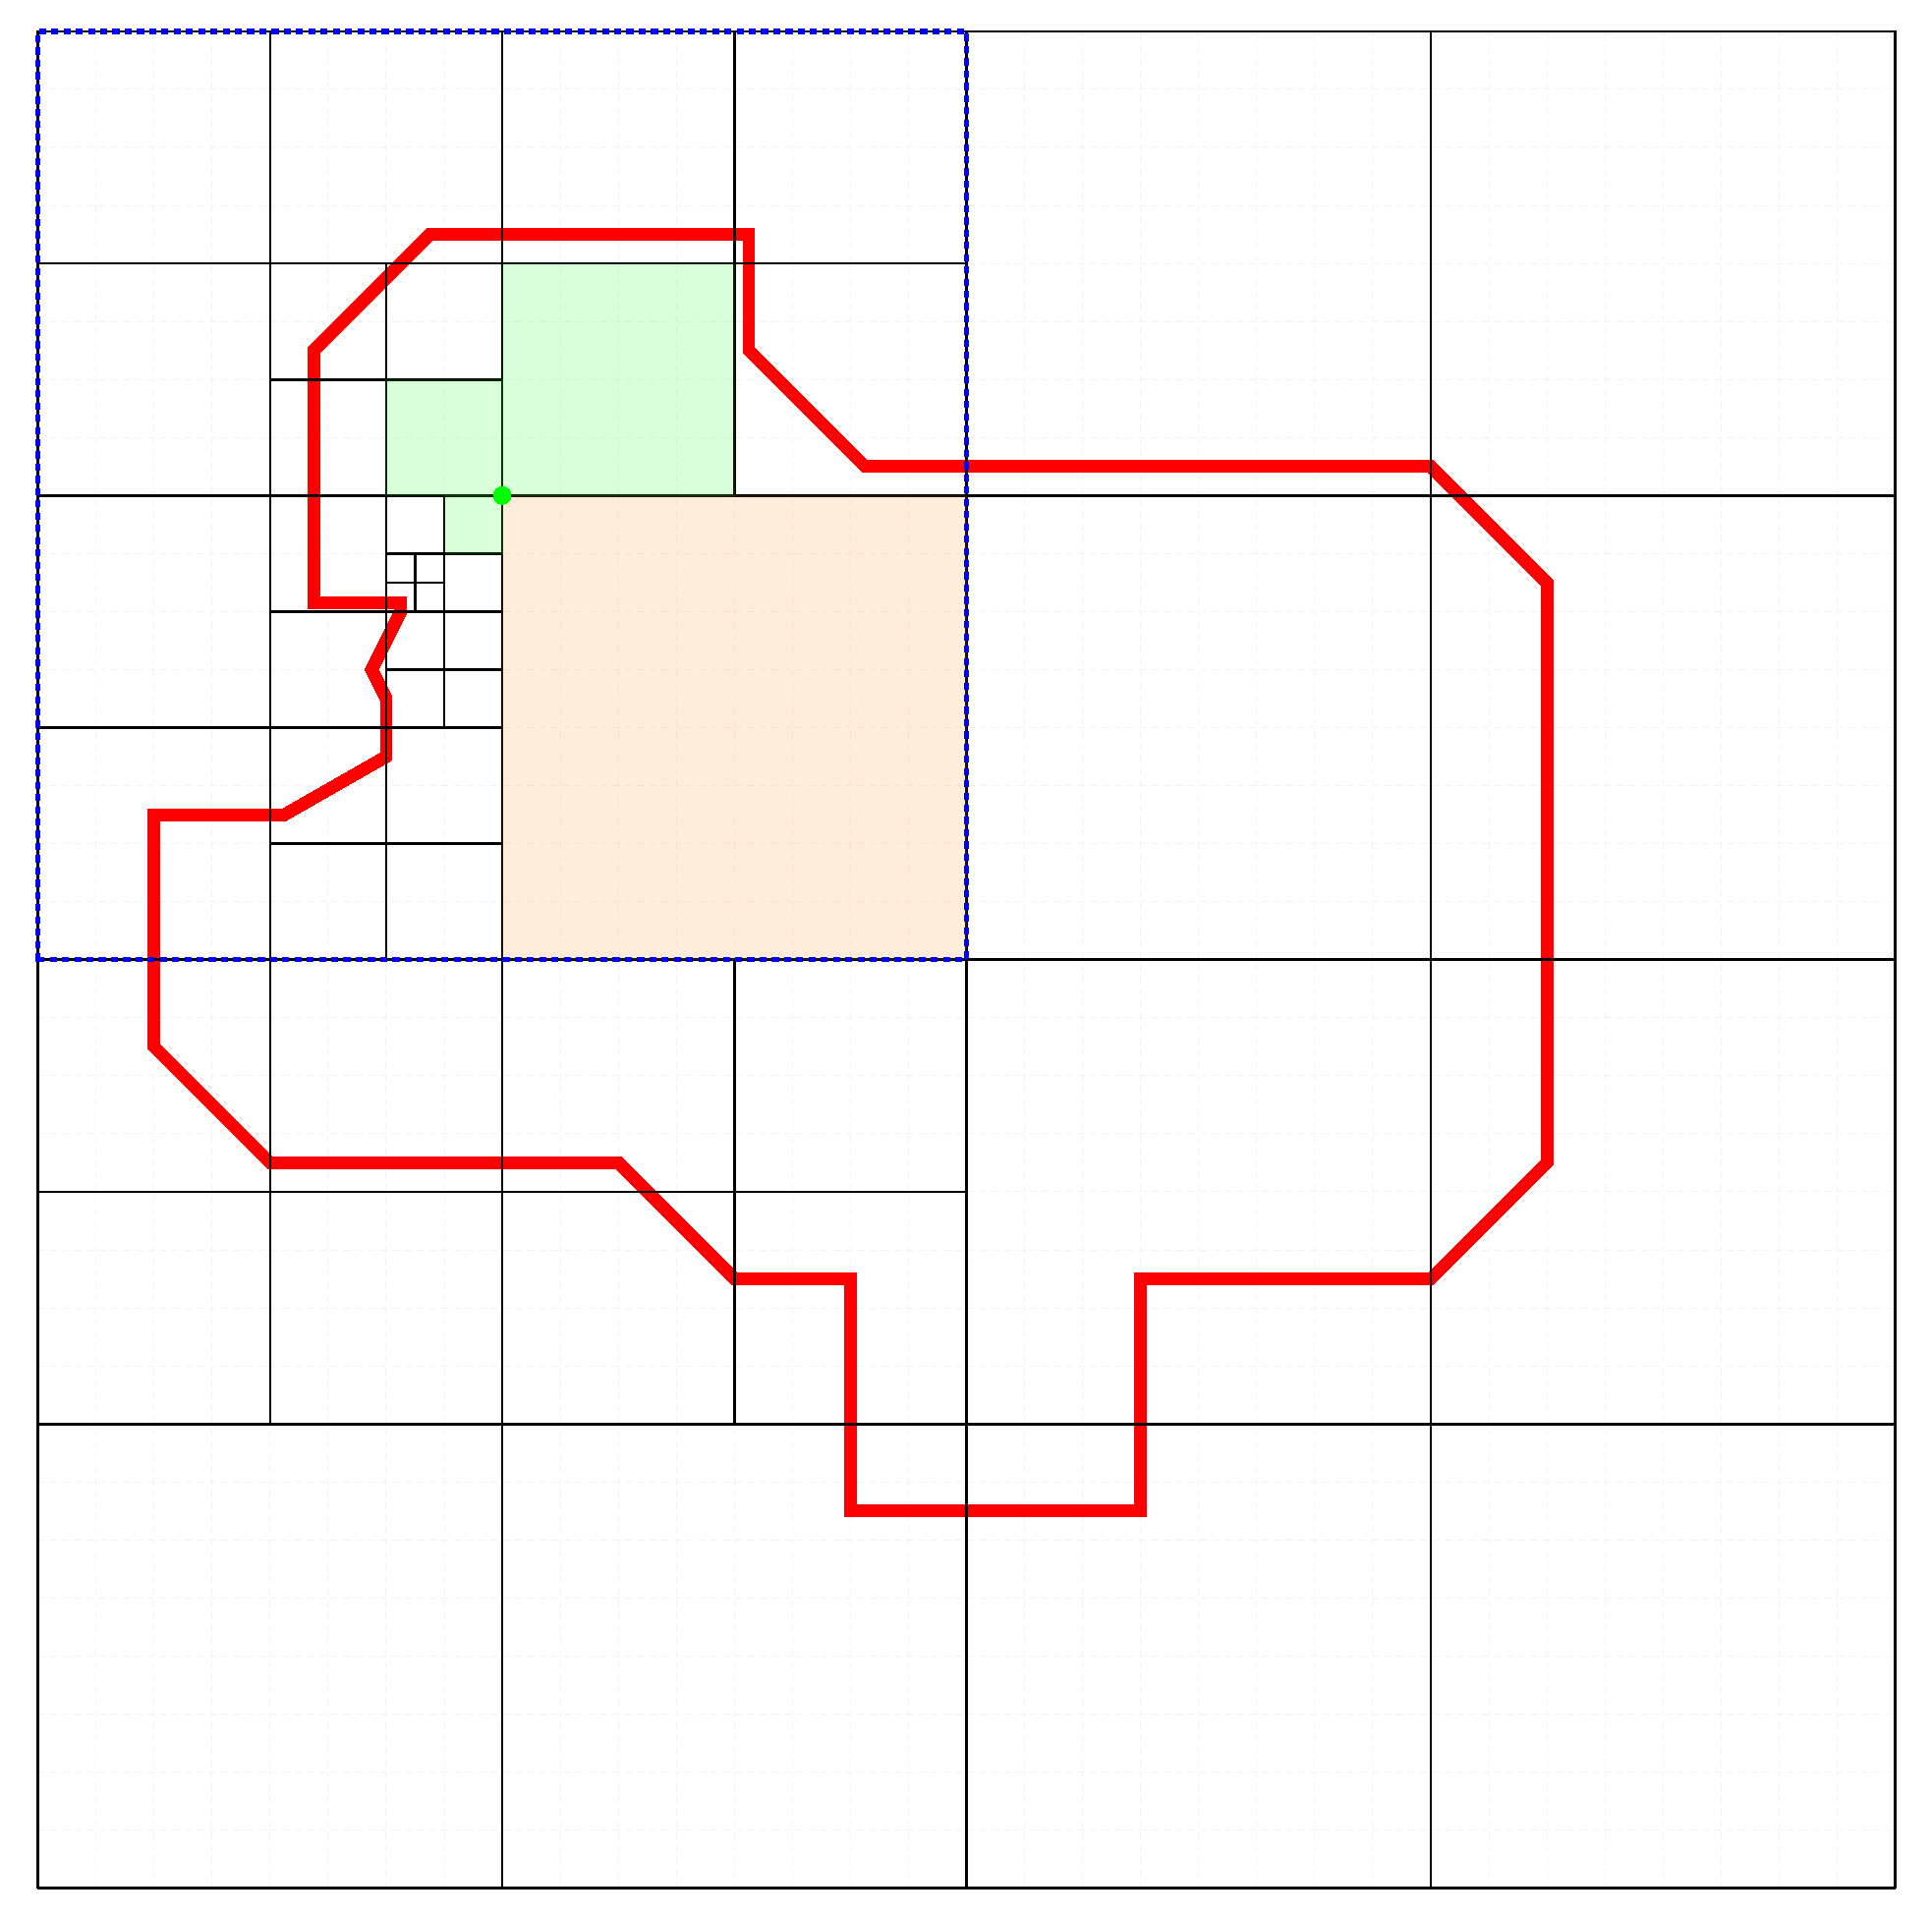
\includegraphics[page=1, width=0.55\linewidth]{Figures/Example}
    \end{figure}
    \begin{figure}[!ht]
        \centering
        \includegraphics[page=2, width=0.55\linewidth]{Figures/Example}
    \end{figure}
    \begin{figure}[!ht]
        \centering
        \includegraphics[page=3, width=0.55\linewidth]{Figures/Example}
    \end{figure}
\end{document}
